% Template for replying to reviewer comments
%
% Author: Gertjan van den Burg (https://gertjan.dev)
% Source: https://github.com/GjjvdBurg/LaTeXReviewReplyTemplate
% License: MIT
% 
% Command usage:
%
%  - Reply: complete answer to the point raised.
%
%  - Partial reply: partial answer to the point raised. More text may be 
%    needed. Can also imply work on the paper that still has to be done.
%
%  - Todo reply: Used for discussion and/or sketching a reply.
%
%  - Need reply: Signals that a point needs to get a reply.
%
\documentclass[11pt,a4paper]{article}

\usepackage{geometry}
\usepackage[most]{tcolorbox}

% Colors
\definecolor{lightgray}{rgb}{0.9, 0.9, 0.9}
\definecolor{lightyellow}{rgb}{0.98,0.91,0.71}
\definecolor{lightred}{rgb}{0.8,0.4,0.4}

% Boxes
\newtcolorbox{replybox}{colback=lightgray, grow to right by=-10mm, grow to 
	left by=-10mm, boxrule=0pt, boxsep=0pt, breakable, before skip=10pt}
\newtcolorbox{partialbox}{colback=lightyellow, grow to right by=-10mm, grow to 
	left by=-10mm, boxrule=0pt, boxsep=0pt, breakable, before skip=10pt}
\newtcolorbox{todobox}{colback=lightred, grow to right by=-10mm, grow to left 
	by=-10mm, boxrule=0pt, boxsep=0pt, breakable, before skip=10pt}

% Counters
\newcounter{epntcnt}
\newcounter{rpntcnt}
\newcounter{revcnt}

% Environments
\newenvironment{reviewer}{%
	\refstepcounter{revcnt}%
	\setcounter{rpntcnt}{0}%
	\section*{Reviewer \therevcnt}%
}{}
% Editor environment takes an optional argument
\newenvironment{editor}[1][Editorial Decision]{%
	\setcounter{epntcnt}{0}%
	\section*{#1}%
}{}

% Reply Commands
\newcommand{\reply}[1]{%
	\begin{replybox}%
		#1
	\end{replybox}%
}
\newcommand{\partialreply}[1]{%
	\begin{partialbox}%
		Partial reply: \emph{#1}
	\end{partialbox}%
}
\newcommand{\todoreply}[1]{%
	\begin{todobox}%
		Todo reply: \emph{#1}
	\end{todobox}%
}
\newcommand{\needsreply}{%
	\todoreply{This comment needs a reply.}%
}

% Point command differs depending on the environment
\makeatletter
\newcommand{\point}{%
	\medskip\noindent%
	\def\@tmp{editor}%
	\ifx\@tmp\@currenvir \refstepcounter{epntcnt}\theepntcnt\textbf{.}  
	\else%
	\def\@tmp{reviewer}%
	\ifx\@tmp\@currenvir \refstepcounter{rpntcnt}\therpntcnt\textbf{.}  
	\else\fi\fi%
}
\makeatother

% Renew the commands for the point counters to get the formatting we want in 
% both the references and the item labels.
\renewcommand{\therpntcnt}{\textbf{\textup{\therevcnt.\arabic{rpntcnt}}}}
\renewcommand{\theepntcnt}{\textbf{\textup{E.\arabic{epntcnt}}}}

%\setlength\parindent{0pt}
\newcommand{\bft}[1]{\mathbf{#1}}

\usepackage[hidelinks]{hyperref}
\usepackage{natbib}
\bibliographystyle{abbrvnat}
\usepackage{booktabs}
\usepackage{subcaption}

\renewcommand{\thefigure}{R\arabic{figure}}
\renewcommand{\thetable}{R\arabic{table}}

\title{Reply to Reviewer Comments}
\author{Dirk Seidensticker}

\begin{document}
\maketitle

\noindent I very much thank the two referees for their helpful comments and advice. The revisions addressing their comments have substantially improved the paper, though none of its significant results or conclusions have changed.

I have amended the manuscript to fully incorporate all comments made. The main changes are the following:


\begin{itemize}
	\item [-] Two paragraphs were added at the end of the discussion detailing the ramifications of the regional findings of this study for the supra-regional debate of the 'Bantu-Expansion'.
	\item [-] Fig. 2 was expanded with a map detailing the supra-regional scope of the graphs.
\end{itemize}

\noindent The Author\\

\noindent \today.

{\centering \section*{Comments to the author and responses}}

\begin{reviewer}
Reviewer \#1: The current paper is another in a series of new contributions to Central African archaeology that have revitalized the much-needed research there. This particular study brings the analysis of pottery recipes (macro/petrographic) and forming techniques (Macro-traces/x-radiographs) to the Pikunda-Munda pottery style, which is the oldest currently known style in the northern Congo Basin in order to produce a comparative analysis. Thus, the geographical focus is an important one, as some (Bostoen, Grollemund, etc.) claim the region as one of the major pathways of the Bantu Expansion - something that is far from certain. Thematically, it is likewise fantastic to see methods new to the region being applied to Central African assemblages. These are long-overdue and significant contributions. The manuscript is ideal for publication in AAR.

Overall, the manuscript is well written and organized and is close to being ready for publication. I only have one major comment and several other smaller comments/edits that should be addressed prior to publication.

For the 'major' comment: It appears that a large portion of the introduction is a bit incongruous with some of the data presented and discussed in the remainder of the paper. Indeed, it appears that some of the points there are somewhat contradictory. In particular, the idea that the period of 'Low Activity' is necessarily taken as evidence for an abrupt discontinuity between EIA and LIA populations and therefore opposes the idea of a connection between the early pottery-producing communities and modern Bantu speakers, while there are clearly some continuities discussed in the rest of the manuscript. Although I am somewhat sympathetic to the claims of the author, they are significant and therefore should be made clearer. I propose a few areas where the author could add or clarify some thoughts:

\point Firstly, the author mentions that the Congo Basin was not completely depopulated during the 7-10th centuries - a period of 'Low Activity' is not a period of no activity. This, inherently, leaves room for possible continuity as communities are still present - which I am pretty sure most of the scholars cites here would agree with. Does the author envision a 'spread over spread' event of LIA Bantu-speakers over/integrating EIA populations? Does that author hypothesize that these EIA populations Bantu-speaking? If the author is going to critique the current models of the Bantu Expansion here, they need to address this (or at least give two or three sentences providing some thoughts on how their model differs).

\begin{figure*}[p]
	\centering
	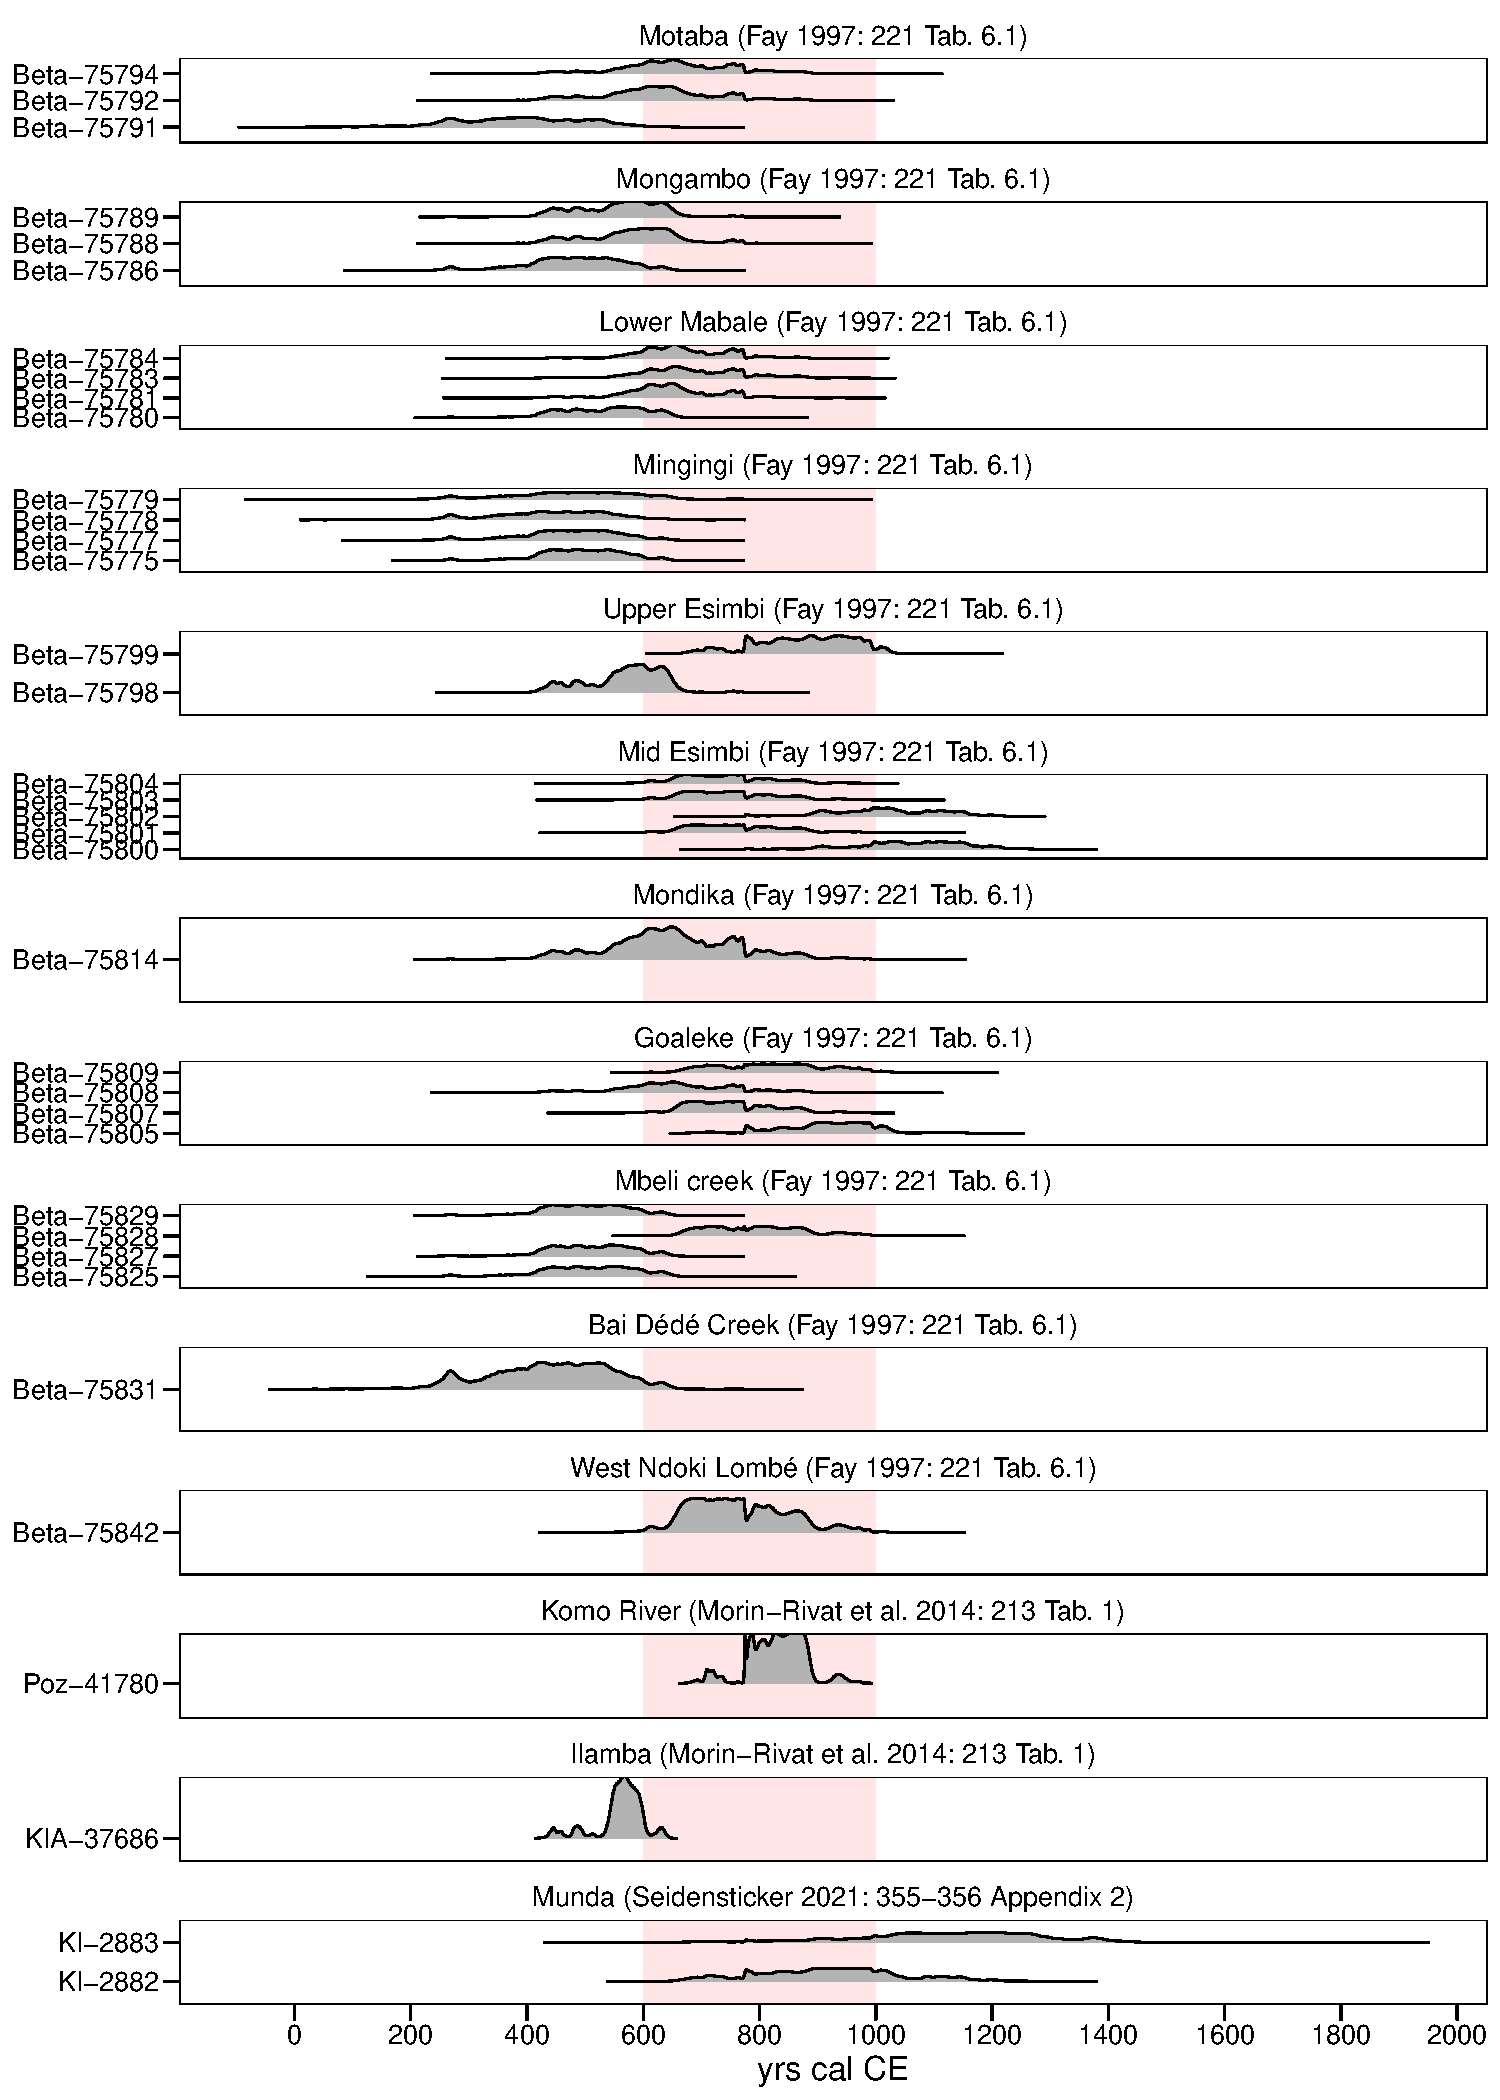
\includegraphics[width=.9\textwidth]{output/rev_fig_c14_wCB_hiatus.pdf}
	\caption{Calibrated ages of radiocarbon dates from the western Congo Basin \citep[region E in][Fig. 1]{Seidensticker.2021} that date into the 7th to 10th century CE, the proposed periods of lower human activity throughout Central Africa \citep{Seidensticker.2021}. Sites are sorted from North to South.}
	\label{fig:rev_fig_c14_wCB_hiatus}
\end{figure*}

\reply{Distinguishing periods of 'low activity' versus those with 'no activity' is for sure no easy feat with the available records being difficult to interpret, which led to quite profound differences in opinion between scholars \citep[cf.][]{Clist.2023a}. The supra-regional study by \citet{Seidensticker.2021} corroborated earlier regional assessments by \citet{Oslisly.1998} and the similar analysis by \citet{deSaulieu.2021a}, in that the communities living in the equatorial rainforests of Central Africa in the 5th--6th century CE must have undergone some kind of crisis leading to a considerable reduction of signals for human activity in the archaeological record. \citet[Fig. S4]{Seidensticker.2021} distinctly debate the role of relic populations. The present paper does not offer the scope to critique the 'current models of the Bantu Expansion', although the author's stand concerning connecting modern language data with archaeological finds has been published recently \citep{Seidensticker.2024}. Nonetheless, I am grateful for the remarks by the reviewer and have streamlined the text to better depict that, while at a supra-regional scale a 'setback' of human activity can be identified, for the western Congo Basin, the region of the Pikunda-Munda style pottery, a complete hiatus, and end of the tradition of Pikunda-Munda potters' communities must be presumed. The similarity in vessel shape with the Mobaka style, which the reviewer noted below (see \ref{rev1:clays}), is inexplicable, but should not be over-interpreted as sign of continuity either; especially taking into account the 1.500 year difference between the two styles. The few Mobaka bowls were unfortunately not studied in term of shaping techniques and thus it must remain an unsettled question if these bowls were produced following a \textit{chaîne operatoire} similar to that of Pikunda-Munda potters'. Thus, the pottery inventories themselves offer no signs that any traits of the Pikunda-Munda potters' knowledge persisted. Concerning the chronometric records from the western Congo Basin in particular: while 36 radiocarbon dates from 14 locations in the western Congo Basin \citep[region E in][Fig. 1]{Seidensticker.2021} fall -- after calibration -- into the 7th to 10th century CE (Fig.~\ref{fig:rev_fig_c14_wCB_hiatus}), out of these, only the two radiocarbon dates from an iron furnace or smith's hearth at Munda \citep[311--321]{Seidensticker.2021e} are associated with archaeological finds. These two dates \citep[Tab.~1: KI-2882 \& KI-2883]{Seidensticker.2024} are problematic though: not only do these two dates entail substantial standard errors of 110--180 years, a stratigraphically older, directly adjacent pit dates younger than the 16th century CE \citep[Tab.~1: KI-2884, Tab.~2: RICH-30865 \& RICH-30866]{Seidensticker.2024}. \citet[319--321]{Seidensticker.2021e} attempted to interpret this conundrum with the stratigraphically younger metallurgy feature producing considerable older radiocarbon dates than the stratigraphically older pit and suggested that a potential old-wood-effect affected the radiocarbon dates KI-2882 \& KI-2883. That the novel dates RICH-30865 \& RICH-30866 corroborated the younger date KI-2884 from the stratigraphically older pit further substantiated the notion that the difference in radiocarbon ages between the two, partially overlapping features is no mere lab-error. With the stratigraphic feature being quite straightforward \citep[315 Fig. 151C]{Seidensticker.2021e}, it must be accepted that the feature that yielded radiocarbon samples KI-2882 \& KI-2883 is in fact younger than the 16th century CE and that the two dated charcoals do not represent the age of the feature. Thus, the author would not consider them representative of human activity during the period of overall reduced human activity in the equatorial rainforest of Central Africa \citep{Seidensticker.2021}. The remaining 34 radiocarbon dates that fall into the 7th to 10th century CE (Fig.~\ref{fig:rev_fig_c14_wCB_hiatus}) were obtained during paleo-ecological surveys. While \citet{Seidensticker.2021} considered those dates as weak proxies for human activity, due to them originating from finds of \textit{Elaeis guineensis} and thus interpreted as human induced signal in the rainforest vegetation by \citet{Fay.1997}, and included them into the modeling, they lack explicit associations with human made objects. The author interprets the patchy evidence from the western Congo Basin as follows: while the analysis of radiocarbon dates points towards some relic communities still populating at least parts of the region, the specific knowledge of potters' producing Pikunda-Munda style pottery dissapears, as no subsequent pottery shows any reminiscence of this older pottery. The similarities between the Pikunda-Munda pottery and younger pottery found in the region, such as the styles Ngombe or Ebambe, are on a level (similarities in clay sourcing and preparation strategies; see \ref{rev1:clays}) at which these younger styles could have inherited these traits from contemporary potters' communities in the adjacent Inner Congo Basin; none of those traits are unique to the Pikunda-Munda pottery.}\label{rev1:continuity1}

\point Furthermore, isn't the fact that both the Pikunda-Munda "style" and many of the LIA "styles" that later emerge in the region have their origins in the Equator-Co tradition (P8 L13-14) some evidence of continuity? At least within tradition? The phylogenetic use of tradition here, sensu Wotzka, would suggest that if they are within the same tradition they are by definition related (thus necessarily a continuity).

\reply{The Equator-Co-Tradition acts as a more stable 'anchor' for the heritage of potting practices in the region for sure. The reviewer reports the notion of \citet{Wotzka.1995} concerning '(phylo)genetically' linked pottery styles, meaning those that show reminiscent morphological or ornamental features, as part of a tradition and multiple related traditions with a common root as a co-tradition, following \citet{Rouse.1957}. While the author followed the same approach in prior studies \citep{Seidensticker.2021e}, it is not without issues: for example is the chronological connection between the latest pottery styles pertaining to the Early Iron Age in the Inner Congo Basin (Bokuma \& Lindonga) and the earliest styles attributed to the Late Iron Age (Bondongo \& Longa) difficult to assert \citet{Seidensticker.2024}. While prior estimates by \citet[121--128]{Wotzka.1995} placed the Longa style in-between these two phases, a novel AMS-date from Ngombe \citet[Tab.~2: RICH-30867]{Seidensticker.2024} corroborated the younger of the three radiocarbon dates for Longa style pottery. Subsequently, it must be proposed that Longa style pottery only dates to after the 10th century CE \citet{Seidensticker.2024}, leaving three centuries with no pottery styles accounted for in the Inner Congo Basin. The notion of \cite{Wotzka.1995}, who can see no influences from surrounding regions, must partially be attributed to the circumstance that at the time of analysis, no studies have taken place on pottery from regions bordering the Inner Congo Basin. In light of these new data, a critical review of the sequence of the Inner Congo Basin and especially the putative continuity between pottery styles pertaining to the Early and Late Iron Age is necessary. Such a review must include reconstructions of potters' \textit{chaînes opératoires} to deduce transfer of knowledge. In summary, while the Equator-Co-Tradition constitutes the -- at least somewhat 'stable' -- backbone of a genealogical network for trans-generational knowledge transfer among potters communities in the region, novel research and data raise chronological issues that need to be solved before claiming continuities.}

\point Likewise, other continuities exist in the results of the current study. The use of the same clay sources/recipes by EIA potters and those at LIA sites along the lower Sangha and Likawala-aux-Herbs, for example (P14 L24-26). In addition, the similar vessel shapes of the Pikunda-Munda group and the later, LIA, Ngombe/Longa and Mobaka styles from the Sangha/Inner Congo Basin and Likwala-aux-Herbs respectively (P23 L42-43). 

\reply{Clay procurement and processing strategies are as early stages of the \textit{chaîne operatoire} only superficially more reliable indicators for knowledge transfer than stylisticly driven rationales, like the one proposed by \citet{Wotzka.1995}. It must be noted that due to the lack of studies focused on available clay sources, the variability of clay sources in proximity of potters' villages remains unknown. Without this knowledge it remains speculative to what degree potters were limited by the available resources in their immediate surrounding. While potters' can be quite opportunistic and "satisfy themselves with a very wide spectrum of clays" \citet[148]{Gosselain.1997}, "most African potters collect their clay within a 3 km radius from the place where they live and/or practice the craft" \citet[35]{Gosselain.2005}, which matches the patterns found by \citet[452]{Whitbread.1986}. This means that the selection criteria for the clays used, while being embedded within the socio-historical background of a potter, are not completely uncoupled from environmental constraints and thus not purely socially deterministic.	Somewhat more refined research on this topic by the author has been presented in the summer of 2024 \url{https://youtu.be/KoSq-O5N_tw} and worked into a scientific paper that is destined to be submitted soon. More specifically: while the pottery at Munda indicated similar or even the same sources have been used during the Early and Late Iron Age and potters in Pikunda approach very different sources during the Early Iron Age than in the Late Iron Age, the situation along the Luilaka river, between the villages of Monkoto and Wafanya, revealed to be much more diverse than initially expected. There, sherds dating into the Early Iron Age showed a petro-fabric indicative of the usage of un-tempered fluvial clays, very similar to the situation in Munda. Samples obtained from locations on the \textit{terra firme}, at around 3.2-3.7~km distance from the Luilaka river, dating into the period of 'low activity' show the usage of non-fluvial clays that were tempered with plant matter and grog, the latter derived from pottery produced from fluvial clays. Afterwards, at the onset of the Early Iron Age, potters 'revert' back to the recipe of the Early Iron Age and continue to use fluvial clays without any tempering. All these novel data points are currently to sparse to deduce a reliable anti-thesis to established concepts though. Concerning the raised similarities in vessel shapes, especially between Pikunda-Munda and Mobaka bowl, please see \ref{rev1:continuity1}. The mentioned similarity between vessels of the styles Longa \citep[121--128]{Wotzka.1995} and Ngombe \citep[125--128]{Seidensticker.2021e} are purely regarded as sign of contemporaneity, and thus 'horizontal' and not 'vertical' connectivity.}\label{rev1:clays}

\point While I understand why the author is using the clear evidence for this period of 'Low Activity' as evidence for a degree of discontinuity, in order to use this as evidence for a larger point (which the author touches on) about the nature of the Bantu Expansion they need to address these seeming contradictions - the presence of continuity in recipes/clay sources and some pottery forms, and their categorization into the same 'tradition'. Likewise, they should add a few lines in the conclusion/discussion where they fold the actual results of the present study into this argument. Otherwise, it may possibly be seen as a non sequitur. 

\reply{The text has been amended accordingly and the individual points of critique were assessed above (\ref{rev1:continuity1}--\ref{rev1:clays}). See also \ref{rev:anti-bantu} for the author's stand on the debate of the issue of mixing linguistic hypotheses with empirical historical data.}

\noindent A few smaller comments:

\point There are several small editorial errors that need to be fixed - missing spaces in citations (P3 L42), an errant question mark (P3 L44), "Eggert (2014)" should be (Eggert 2014) (P3 L47), the wrong inverted comma at the beginning of a word (P6 L10), question marks in citations (P18 L37), "one sherds" (P13 L35), invert "are they" (P23 L22), etc.

\reply{Many thanks for the thorough and careful review and detecting these editorial errors. All noted errors were corrected and the text was again proof read to fix additional editorial errors. Only the style of quotation marks could not be rectified as those are linked to the \LaTeX{} style of AAR.}

\point P6 L9-15 Is the argument that this apparent disruption in settlement is evidence for a much later (and thus faster) Bantu Expansion? Is the argument then that the EIA groups were non-Bantu speaking? There seem to be a lot of "raising questions" and "challenging assumptions" without proposing a counter hypothesis to the things being questioned/challenged (even in the conclusion/discussion).

\reply{The established paradigm of the Bantu-Expansion brought forward by the reviewer is based on the notion that modern languages and material culture of prehistoric communities could be superimposed easily. This claim and the underlying assumption have been criticized for multiple decades \citep[a non representative selection of studies:][]{deMaret.1989,Robertson.2000,Eggert.2005,Eggert.2016a}. As mentioned earlier, the author's position was published recently \citep{Seidensticker.2024} (see also \ref{rev1:continuity1}). With the focus of this study being the disappearance of a distinct pottery tradition in the western Congo Basin at the end of the Early Iron Age -- in the 5th/6th century CE --, shifting the debate towards the impact similar 'losses of knowledge' during the prehistory of sub-Saharan Africa might have had on the debate of the 'Bantu-Expansion' might be too much to ask. The author holds a critical view on published reconstructions of the Bantu-Expansion \citep{Bostoen.2015,Grollemund.2015,Grollemund.2023,Koile.2022} as these are -- again in the view of the author -- entail assumptions that are not discussed, but that are vital for the models acceptance. 1) The main driver of the supra-regional dissemination of the modern Bantu-languages is considered to has been demic diffusion based on results by population genetics \citep{Pakendorf.2011}. Recent critical assessments conclude that "the structure of ancient populations cannot be robustly reconstructed based solely on genetic data from present-day people" due to disruptions by "demographic transformations", including "colonialism, imperialism, enslavement, and modern sociopolitical reorganization" \citet[1]{Lipson.2022}. But the rare aDNA samples from sub-Saharan Africa -- exemplary 
\citet{Prendergast.2019} for eastern Africa and \citet{Gretzinger.2024} for southern Africa -- indicate genetic ancestry linked to West Africa farmers to date around or younger than the 10th century CE. In both regions are pottery finds that have been linked to the 'Bantu-Expansion' \citep{Huffman.2007} considerably older though. A novel and extensive review of the available genetic data by \citet{FortesLima.2024} found only "a marginally significant negative correlation between linguistic and genetic data is observed after controlling for geography" lead the authors to conclude that this "could point to separate histories underlying the genetic and linguistic data that could involve secondary, and potentially more localized, spread waves". \citet{FortesLima.2024} note that the "linguistic data may represent only the latest spread event". In summary do these newer assessment of population geneticists and hopefully increasing aDNA data point -- again in the view of the author -- urge caution in accepting the underlying assumption that reconstructing modern language data reveals prehistoric demic diffusion paths' in sub-Saharan Africa. 2) The chooses statistical approach by \citep{Bostoen.2015,Grollemund.2015,Grollemund.2023,Koile.2022} of phylogentic modeling will always result displaying an output that suggests parent-child-relationships within the dataset. The method is unable to detect cross-entity knowledge-transfer or extinction-events \citep[cf.][]{Pagel.2020}. 3) The concept of communal mobility that \citep{Bostoen.2015,Grollemund.2015,Grollemund.2023,Koile.2022} apply as basis for their model on the dispersal of modern speech communities seems to equate today's localities of languages with the initial 'arrival', while oral-historical records \citep[for example by][80--86]{Vennetier.1963} reports considerable mobility of communities in the not so distant past. 4) To use archaeological phenomena as done by \citep{Bostoen.2015,Grollemund.2015,Grollemund.2023} to make assumptions about the deep history of a modern language dispersal requires a continuity between the precise prehistoric community used as reference and the modern communities speaking the studied language. For none of the chosen 'calibration points' such a direct historical trait can be deduced in the archaeological record. For examples it remains illusive why \citet[SI p.~2]{Grollemund.2015} equates the initial off-branching of narrow Bantu (node 1) in the Cameroon-Nigeria homeland with the archaeological inventories of the lower horizon of the Gray Ash layer from the site of Shum Laka, representing the second phase of the "Stone to Metal Age" (SMA) or "Ceramic Late Stone Age" and dating into the 3rd to 2nd millennium BCE \citep[226--231, 243]{Lavachery.2001}. During that phase the microlithic quartz industry, dominating the late Pleistocene deposits \citep[172 Fig.~4]{Cornelissen.2003,Cornelissen.2017}, is slowly declining, while a macrolithic flake and blade industry on basalt, which occurs in smaller numbers in older deposits as well, becomes more prevailing \citep[169 Fig. 1]{Cornelissen.2003,Cornelissen.2017}. Pottery, while already present in the older deposits of the upper horizon of the Ochre Ash layer and dating into the 5th to 4th millennium BCE \citep[224--225 Fig.~4.2–3]{Lavachery.2001}, is now more prominent and decorated with grooves and impressions, including rocker zig-zag \citep[231--232 Fig.~8]{Lavachery.2001}. It must be stressed that Shum Laka represents the only site in the wider region of the putative homeland of the Bantu languages, the border area of Nigeria and Cameroon, that has been studied in detail. The deciding factor of \citet{Grollemund.2015} for 'selecting' the specific deposits at Shum Laka as an archaeological 'calibration point' for their phylogentic language tree seems to be neither quantitative nor qualitative. And while \citet[SI p. 2]{Grollemund.2015} allege that "small immigrant communities from further north" introduced pottery and Benue-Congo languages, more recent genetic analyses from four burials at Shum Laka, dating into the early 6th and late 2nd millennium BCE, showed that the genetic profiles of the occupants of the site "are very different from those of most speakers of Niger–Congo languages today, which implies that these individuals are not representative of the primary source population(s) that were ancestral to present-day Bantu-speakers" \citep[5]{Lipson.2022}. \citet[SI p.~2]{Grollemund.2015} date the subsequent node of Bantu languages, the off-branching of Mbam-Bubi languages, in the younger half of the 2nd millennium BCE based on the earliest occurrence of markers for 'sedentism' at Obobogo in southern-central Cameroon \citep{deMaret.1982,deMaret.1992}. It must be noted that final analyses from the site of Obobogo are still pending. \citet{Claes.1985} provided some initial results, but not a conclusive analysis of the available data. \citet[SI p.~2]{Grollemund.2015} associate the third mayor branching-off point of the East Bantu languages with the emergence for Urewe ceramics in the Great Lakes region of East Africa. All these choices together perpetuated the trope that early Bantu-speakers can be equated with the earliest pottery production in a given region \citep[355, 362, 364]{Bostoen.2015}. In a nutshell, the procedure of adopting opportune archaeological results for underpinning linguistic reconstructions by \citet{Grollemund.2015,Grollemund.2023} and \citet{Bostoen.2015}, which was subsequently adopted by \citet{Koile.2022} without any critical review, represents another facet of a long-standing tradition in circular reasoning \citep{Ehret.1973,Phillipson.1976,Phillipson.1976b,Phillipson.1977a,Heine.1977}. 5) \citet[SI p. 3]{Grollemund.2023} clearly states that constraints were introduced into the model until "simulated routes [...] coincide[d] with the the savannah corridor", which makes the published results a result of the mentioned circular reasoning. The existing approaches on the 'Bantu-Expansion' induce "procedural puzzles" and fail at linking linguistics with "the authentic material evidence of archaeology" \citep[88]{Eggert.2016a}. In consequence it can only be reiterated that "non-written languages do not leave material traces" \citep[85]{Eggert.2016a}.}\label{rev:anti-bantu}
	
\point P12 L30: I would be careful to claim that sponge spicule rich pottery is rare in Africa, as there have been exceedingly few studies in these regions to clarify if they are common or not (which is indeed one of the reasons why the current study is so enlightening).

\reply{The sentence in question has been rephrased to better depict that: "Sponge spicules rich pottery is rarely documented in pottery from sub-Saharan Africa though." Furthermore, a reference to the, albeit old overview of \citet{Drost.1967} was introduced to highlight the difference between the wide use of fluvial clays among modern potters against the empirical evidence from archaeological sources.}

\point P18 L36: I do not think this is a fair assessment of all archaeological studies of pottery - "as tools" (per Braun 1983) - prior to the 2000s. Socio-cultural studies of pottery have long pre-dated Roux and Gosselain. For instance, a contemporary study in Mali by S. McIntosh (1995) did just that.

\reply{The author concurs with the reviewer in that the socio-historical setting of potters' has been debated well in advance of the cited literature. The sentence in question has been rephrased and the reference to \citet{McIntosh.1995} was added to reflect that there is little replacement of ideas but rather a side-by-side.}

\end{reviewer}

\begin{reviewer}
\end{reviewer}
	
\begin{reviewer}

Reviewer \#3: This well-conceived and very well-written paper offers a detailed synthesis on the chronological extension of multiple pottery tradition in the Western Congo Basin at the end of the Early Iron Age, with a special focus on the Pikunda-Munda group. The latter is one of the oldest pottery tradition documented in the Congo Basin, emerging in the last centuries BCE but extinguishing around the 5th-6th c. CE. The author carefully reconstructs the range of technical operations implied in the production of these ceramic containers, from petrographic observations in thin-sections to macroscopic and X-ray analysis to precise roughing-out and preforming techniques.

This precise methodology perfectly serves the definition of a more precise regional scenario, interrogating the fluctuation of population dynamics in that region.

It is an important contribution that renew and clarify our understanding of ancient Central African pottery traditions and their related technologies. The attention given by the author to the presentation of data prevent from any important remarks regarding the constitution of the article. Technical features are indeed precisely exposed, as well as the corpus of pottery studied itself (provenance, sample, type of analysis conducted, reference to previous publication).

It must be stated that this version of the manuscript already benefited from previous discussions with the author, explaining why I see no conflict in waiving my anonymity. The author strongly strenghtened the presentation of the corpus as well as the technological characteristics of pottery traditions.

Therefore, considering the important work presented in this study and the regional scope of its analysis, maybe the author could further detail his perspectives in the conclusion, thus emphasizing more again the importance of technological studies in the reconstruction of past cultural dynamics or future paths in the archaeology of settlements in the (Western) Congo Basin.

Adrien Delvoye

\reply{Many thanks, also for the previous discussions, which strongly helped to refine this manuscript. As the recommendation to refine the text in terms the wider ramifications this regional study has are similar to the points raised by reviewer 1, I want to draw your attention at my extended remarks above.}

\end{reviewer}

%\bibliographystyle{spbasic}
\bibliography{references.bib}

\end{document}
